\documentclass[12pt, a4paper]{report}
\usepackage{graphicx}
\usepackage{hyperref}
\usepackage[left=1in, right=1in, top=1in]{geometry}
\title{Coursera Capstone Project - Week 5\\ \textbf{Finding US cities similar to Phoenix} }
\author{Bhaumik Choksi}

\begin{document}
	\maketitle
		
	\section*{Introduction}
	A city can be defined broadly as a collection of various commercial, governmental and residential properties. Identifying similar cities can have many potential applications. Lawmakers, businesses and even common people can use these relationships to draw relevant insights. 
	
	This project aims to leverage location and venue data in order to identify cities similar to a given city (Phoenix, Arizona in this case). 
	
	
	\section*{Business Problem}
	Given a city, can we use the data about the nearby venues to identify other cities that are similar to the given city in terms of the composition and availability of these venues.
	
	More specifically, \textit{what cities in the US are similar to Phoenix in terms of venues}? 

\newpage

\section*{Description of the data}
I will be using data from two different sources for this project - Foursquare and the US Cities Dataset. The Foursquare API provides data about the venues whereas the US Cities Dataset provides city names and location coordinates. 

\subsection*{Foursquare API}
Website: \href{https://developer.foursquare.com/docs/api/venues/details}{https://developer.foursquare.com/docs/api/venues/details}
\newline
The Foursquare Places API allows users to get details about nearby venues for a given location. I've used this API to get the following details about 10 nearby venues for a given city:
\begin{enumerate}
	\item Venue Name
	\item Venue Latitude
	\item Venue Longitude
	\item Venue Category (Short name)
\end{enumerate}

\subsection*{US Cities Dataset}
\begin{itemize}
	\item Original Name: 1000 Largest US Cities By Population With Geographic Coordinates
	\item Website: opendatasoft.com
	\item Source: \href{https://public.opendatasoft.com/explore/dataset/1000-largest-us-cities-by-population-with-geographic-coordinates/export/?sort=-rank&dataChart=eyJxdWVyaWVzIjpbeyJjb25maWciOnsiZGF0YXNldCI6IjEwMDAtbGFyZ2VzdC11cy1jaXRpZXMtYnktcG9wdWxhdGlvbi13aXRoLWdlb2dyYXBoaWMtY29vcmRpbmF0ZXMiLCJvcHRpb25zIjp7InNvcnQiOiItcmFuayJ9fSwiY2hhcnRzIjpbeyJhbGlnbk1vbnRoIjp0cnVlLCJ0eXBlIjoiY29sdW1uIiwiZnVuYyI6IkFWRyIsInlBeGlzIjoicmFuayIsInNjaWVudGlmaWNEaXNwbGF5Ijp0cnVlLCJjb2xvciI6IiNGRjUxNUEifV0sInhBeGlzIjoiY2l0eSIsIm1heHBvaW50cyI6NTAsInNvcnQiOiIifV0sInRpbWVzY2FsZSI6IiIsImRpc3BsYXlMZWdlbmQiOnRydWUsImFsaWduTW9udGgiOnRydWV9}{Click here}
	\item Reference: \href{https://gist.github.com/Miserlou/c5cd8364bf9b2420bb29#file-cities-json}{Miserlou on GitHub} 
	\item Disclaimer: I do not own any part of this dataset. All copyrights belong to their respective owners. 
\end{itemize}
I will be using the following columns from this dataset:
\begin{enumerate}
	\item City
	\item Rank
	\item Coordinates 
\end{enumerate}
\newpage

\section*{Methodology}	
The implementation involves three main phases - pre-processing, clustering, and PCA. Each phase has it's own set of plots and other visualizations. 
\subsection*{Pre-processing}
We start by importing the US cities dataset obtained from opendatasoft.com. We read the CSV file into a pandas dataframe. It contains details about 1000 cities in the United States. In order to simplify plots and to make sure we don't exceed the free API usage limit, I only select the top 50 cities based on population. 

\begin{figure}[h]
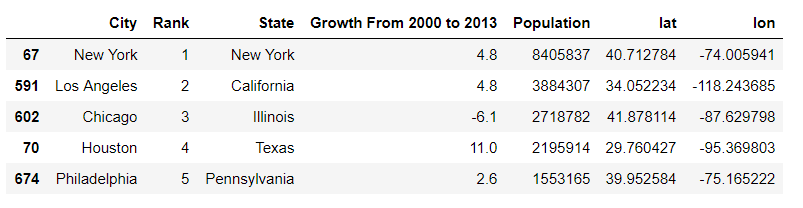
\includegraphics[]{cities_data}
\caption{Cities Data}
\end{figure}

Next, I use the latitude and longitude of each city to obtain the nearby venues using the Foursquare API. I obtain the top 10 venues for each city and extract the name and category of each venue. I store these in a list that is later converted to a dataframe. 

In order to process this categorical data, I one-hot encode the venue categories so that each category is represented as a column. I take the mean of this dataframe to ensure that each category value represents the fraction of the venues that belong to that category for that city. 

\subsection*{Clustering}
In order to identify similar cities, we must cluster the data. Our target here is Phoenix, so we'll be looking for cities that are assigned the same label is Phoenix. 

I start by importing Kmeans from the scikit-learn package. I cluster the one-hot encoded data into 5 clusters. I decided to pick k=5 since we're working with 50 cities, so that would give us 5 clusters with approximately 10 cities per cluster. 

The kmeans labels are stored in the dataframe along with the one-hot values. 

\subsection*{PCA}

\section*{Results}

\section*{Discussion}

\section*{Conclusion}

\end{document}